\documentclass{article}
\usepackage{adjustbox}
\usepackage{float}
\usepackage{textcomp}
\usepackage{graphicx}
\graphicspath{{images/}}
\usepackage{booktabs}
\usepackage{color}
\usepackage{verbatim}
\usepackage{listings}
\usepackage{underscore}
\setcounter{secnumdepth}{5}
\usepackage[bookmarks=true]{hyperref}
\author{Roberto Clapis (841859), Erica Stella (854443)} 
\date{\today}
\title{Politecnico di Milano
	\\A.A. 2015\@-\@2016
	\\Software Engineering 2: ``myTaxiService''
	\\\textbf{I}ntegration \textbf{T}est \textbf{P}lan \textbf{D}ocument}
\hypersetup{pdftitle={Integration Test Plan Document},    % title
	pdfauthor={Roberto Clapis, Erica Stella},                     % author
	pdfsubject={Integration Test Plan Document},                        % subject of the document
	pdfkeywords={TeX, LaTeX, taxi, ITPD, SoftwareEngineering2}, % list of keywords
	colorlinks=true,       % false: boxed links; true: colored links
	linkcolor=black,       % color of internal links
	citecolor=blue,       % color of links to bibliography
	filecolor=black,        % color of file links
	urlcolor=purple,        % color of external links
}
\begin{document}
\maketitle
\begin{center}
	
\includegraphics{polimi-logo}
\end{center}
\clearpage
\tableofcontents
\clearpage
\section{Introduction}
\subsection{Revision History}
%Record all revisions to the document
\subsection{Purpose and Scope}
%State the purpose and scope of the document
This document describes the Integration Test Plan for the myTaxiService application. It provides a plan referring to how the various components of the software architecture described in the Design Document will be integrated for testing. 
\subsection{List of Definitions and Abbreviations}
\begin{itemize}
	\item \textit{UI:} User Interface. 
\end{itemize}
\subsection{List of Reference Documents}
%List all reference documents, for instance: the project description, the RASD, the Design document, the documentation of any tool you plan to use for testing
\begin{itemize}
	\item The document with myTaxiService's description
	\item myTaxiService's RASD
	\item myTaxiService's Design Document
\end{itemize}
\section{Integration Strategy}
\subsection{Entry Criteria}
%Specify the criteria that must be met before integration testing of specific elements may begin (e.g., functions must have been unit tested).
Before the integration testing, each single module must have been tested to verify its correct functioning according to its specifications.
\subsection{Elements to be Integrated}
%Identify the components to be integrated, refer to your design document to identify such components in a way that is consistent with your design 
According to the Design Document, the components to be integrated are:
\begin{itemize}
	\item Database: 
	\begin{itemize}
		\item Accounts
		\item Active Reservations and Requests
	\end{itemize}
	\item Web Server: 
	\begin{itemize}
		\item DBConnector
		\item APIBackend
		\item WebpageCreator
		\item NotificationModule
		\item HttpHandler
	\end{itemize}
	\item UI:\@
	\begin{itemize}
		\item ClientUI
		\item DriverUI
		\item AdminUI
	\end{itemize}
\end{itemize}
\subsection{Integration Testing Strategy}
%Describe the integration testing approach (top-down, bottom-up, functional groupings, etc.) and the rationale for the choosing that approach
The decided testing approach is bottom-up. %TODO inserire motivazione del perchè
\subsection{Sequence of Component/Function Integration}
%NOTE: the structure of this section may vary depending on the integration strategy you select in Section 2.3. Use the structure proposed below as a non mandatory guide
\subsubsection{Software Integration Sequence}
%For each subsystem: identify the sequence in which the software components will be integrated within the subsystem. Relate this sequence to any product features/functions that are being built up
%TODO che vuol dire relate to any product features/functions that are being built up?
\paragraph{Web Server}
The following images describe how the Web Server's 
components will be integrated for testing.
The arrows represent the order of integration.
\begin{center}
	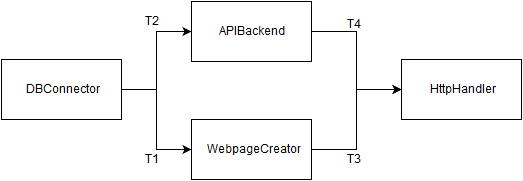
\includegraphics{WebServer1}
	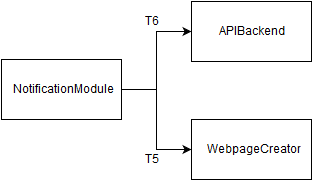
\includegraphics{WebServer2}
\end{center}
\subsubsection{Subsystem Integration Sequence}
%Identify the order in which subsystems will be integrated. If you have a single subsystem, 2.4.1 and 2.4.2 are to be merged in a single section. You can refer to Section 2.2 of the test plan example [1] as an example of what we expect
The following graphs describe how the three 
components of myTaxiService application, 
which are the database, the Web Server and 
the various UIs, will be integrated.
\begin{center}
	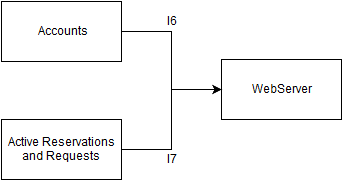
\includegraphics{DBWS}
	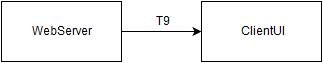
\includegraphics{WSUI1}
	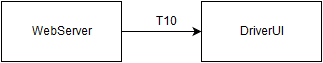
\includegraphics{WSUI2}
	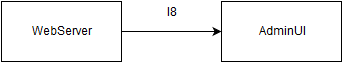
\includegraphics{WSUI3}
\end{center}
\section{Individual Steps and Test Description}
%TODO domanda sui driver
%For each step of the integration process identified above, describe the type of tests that will be used to verify that the elements integrated in this step perform as expected. Describe in general the expected results of the test set. You may refer to Chapter 3 and Chapter 4 of the test plan example [1] as an example of what we expect. (NOTE: this is not a detailed description of test protocols. Think of this as the test design phase. Specific protocols will be written to fulfill the goals of the tests identified in this section.)
\subsection{Test case specifications}
WebServer \rightarrow DBMS
\subsubsection{T1}
\begin{adjustbox}{width=1.2\textwidth}	
	\begin{tabular}{*{2}{c}}
		\toprule
		\textbf{Test Case identifier} & I1T1\\
		\textbf{Test Items} & DBConnector \rightarrow Accounts \\
		\textbf{Input Specification} & Queries to manipulate (creation modification and deletion) of accounts\\
		\textbf{Output Specification} & The actual modifications intended\\
		\textbf{Environmental Needs} & DBMS Driver\\
		\bottomrule
	\end{tabular}
\end{adjustbox}
\subsubsection{T2}
\begin{adjustbox}{width=1.2\textwidth}	
	\begin{tabular}{*{2}{c}}
		\toprule
		\textbf{Test Case identifier} & I2T1\\
		\textbf{Test Items} & DBConnector \rightarrow Active Reservations and Requests \\
		\textbf{Input Specification} & Queries to place/accept/delete reservations and requests, in every possible order of execution\\
		\textbf{Output Specification} & The actual modifications intended and the rejection of the invalid requests\\
		\textbf{Environmental Needs} & DBMS Driver\\
		\bottomrule
	\end{tabular}
\end{adjustbox}

WebServer 
\subsubsection{T3}
\begin{adjustbox}{width=1.2\textwidth}	
	\begin{tabular}{*{2}{c}}
		\toprule
		\textbf{Test Case identifier} & I3T1\\
		\textbf{Test Items} & ApiBackend \rightarrow DBConnector\\
		\textbf{Input Specification} & Perform valid and invalid Requests on the Backend\\
		\textbf{Output Specification} & All and only the queries that should be allowed are executed\\
		\textbf{Environmental Needs} & I1,I2 successful\\
		\bottomrule
	\end{tabular}
\end{adjustbox}
\subsubsection{T4}
\begin{adjustbox}{width=1.2\textwidth}	
	\begin{tabular}{*{2}{c}}
		\toprule
		\textbf{Test Case identifier} & I4T1\\
		\textbf{Test Items} & ApiBackend \rightarrow DBConnector\\
		\textbf{Input Specification} & Perform valid and invalid Requests on the Backend\\
		\textbf{Output Specification} & All and only the queries that should be allowed are executed\\
		\textbf{Environmental Needs} & I1,I2 successful\\
		\bottomrule
	\end{tabular}
\end{adjustbox}

\subsubsection{T7}
\begin{adjustbox}{width=1.2\textwidth}	
	\begin{tabular}{*{2}{c}}
		\midrule
		\textbf{Test Case Identifier} & T7\\
		\textbf{Test Items} & Accounts $\rightarrow$ WebServer\\
		\textbf{Input Specification} & \\ %TODO
		\textbf{Output Specification} & Check if the correct Accounts' methods are called\\
		\textbf{Environmental Needs} & T1 to T6 succeeded\\
		%TODO ha bisogno del driver?
		\bottomrule
	\end{tabular}
\end{adjustbox}
\subsubsection{T8}
\begin{adjustbox}{width=1.2\textwidth}	
	\begin{tabular}{*{2}{c}}
		\midrule
		\textbf{Test Case Identifier} & T8\\
		\textbf{Test Items} & Active Reservations and Requests $\rightarrow$ Web Server\\
		\textbf{Input Specification} & \\ %TODO
		\textbf{Output Specification} & Check if the correct Active Reservations and Requests' methods are called\\
		\textbf{Environmental Needs} & T1 to T6 succeeded\\
		%TODO ha bisogno del driver?
		\bottomrule
	\end{tabular}
\end{adjustbox}
\subsubsection{T9}
\begin{adjustbox}{width=1.2\textwidth}	
	\begin{tabular}{*{2}{c}}
		\midrule
		\textbf{Test Case Identifier} & T9\\
		\textbf{Test Items} & Web Server $\rightarrow$ ClientUI\\
		\textbf{Input Specification} & Typical ClientUI input\\
		\textbf{Output Specification} & \\ %TODO cosa devo controllare?
		\textbf{Environmental Needs} & T7 and T8 succeeded\\
		%TODO driver?
		\bottomrule
	\end{tabular}
\end{adjustbox}
\subsubsection{T10}
\begin{adjustbox}{width=1.2\textwidth}	
	\begin{tabular}{*{2}{c}}
		\midrule
		\textbf{Test Case Identifier} & T10\\
		\textbf{Test Items} & Web Server $\rightarrow$ DriverUI\\
		\textbf{Input Specification} & Typical DriverUI input\\
		\textbf{Output Specification} & \\ %TODO
		\textbf{Environmental Needs} & T7 and T8 succeeded\\
		%TODO driver?
		\bottomrule
	\end{tabular}
\end{adjustbox}
\subsubsection{T11}
\begin{adjustbox}{width=1.2\textwidth}	
	\begin{tabular}{*{2}{c}}
		\midrule
		\textbf{Test Case Identifier} & T11\\
		\textbf{Test Items} & Web Server $\rightarrow$ AdminUI\\
		\textbf{Input Specification} & Typical AdminUI input\\
		\textbf{Output Specification} & \\ %TODO
		\textbf{Environmental Needs} & T7 and T8 succeeded\\
		%TODO driver?
		\bottomrule
	\end{tabular}
\end{adjustbox}
\section{Tools and Test Equipment Required}
%Identify all tools and test equipment needed to accomplish the integration. Refer to the tools presented during the lectures. Explain why and how you're going to use them. Note that you may also use manual testing for some part. Consider manual testing as one of the possible tools you have available.
%TODO Arquillian?
\section{Program Stubs and Test Data Required}
%Based on the testing strategy and test design, identify any program stubs or special test data required for each integration step.
%TODO cosa intende per special data?
\end{document}
